\documentclass[11pt,a4paper,oneside]{report}             % Single-side
%\documentclass[11pt,a4paper,twoside,openright]{report}  % Duplex

%\PassOptionsToPackage{chapternumber=Huordinal}{magyar.ldf}
\usepackage{t1enc}
\usepackage[utf8]{inputenc}
\usepackage{lmodern}
\usepackage{cmap}
\usepackage{amsmath}
\usepackage{amssymb}
\usepackage{enumerate}
\usepackage[thmmarks]{ntheorem}
\usepackage{graphics}
\usepackage{epsfig}
\usepackage{listings}
\usepackage{color}
%\usepackage{fancyhdr}
\usepackage{lastpage}
\usepackage{anysize}
\usepackage[magyar,english]{babel}
\usepackage{sectsty}
\usepackage{setspace}  % Ettol a tablazatok, abrak, labjegyzetek maradnak 1-es sorkozzel!
\usepackage[hang]{caption}
\usepackage{hyperref}

%--------------------------------------------------------------------------------------
% Main variables
%--------------------------------------------------------------------------------------
\newcommand{\vikszerzo}{Bódis-Szomorú András}
\newcommand{\vikkonzulens}{dr.~Konzulens Elemér}
\newcommand{\vikcim}{Elektronikus terelők}
\newcommand{\viktanszek}{Méréstechnika és Információs Rendszerek Tanszék}
\newcommand{\vikdoktipus}{Diplomaterv}

%--------------------------------------------------------------------------------------
% Page layout setup
%--------------------------------------------------------------------------------------
% we need to redefine the pagestyle plain
% another possibility is to use the body of this command without \fancypagestyle
% and use \pagestyle{fancy} but in that case the special pages
% (like the ToC, the References, and the Chapter pages)remain in plane style

\pagestyle{plain}
%\setlength{\parindent}{0pt} % áttekinthetőbb, angol nyelvű dokumentumokban jellemző
%\setlength{\parskip}{8pt plus 3pt minus 3pt} % áttekinthetőbb, angol nyelvű dokumentumokban jellemző
\setlength{\parindent}{12pt} % magyar nyelvű dokumentumokban jellemző
\setlength{\parskip}{0pt}    % magyar nyelvű dokumentumokban jellemző

\marginsize{35mm}{25mm}{15mm}{15mm} % anysize package
\setcounter{secnumdepth}{0}
\sectionfont{\large\upshape\bfseries}
\setcounter{secnumdepth}{2}
\singlespacing
\frenchspacing

%--------------------------------------------------------------------------------------
%	Setup hyperref package
%--------------------------------------------------------------------------------------
\hypersetup{
    bookmarks=true,            % show bookmarks bar?
    unicode=false,             % non-Latin characters in Acrobat’s bookmarks
    pdftitle={\vikcim},        % title
    pdfauthor={\vikszerzo},    % author
    pdfsubject={\vikdoktipus}, % subject of the document
    pdfcreator={\vikszerzo},   % creator of the document
    pdfproducer={Producer},    % producer of the document
    pdfkeywords={keywords},    % list of keywords
    pdfnewwindow=true,         % links in new window
    colorlinks=true,           % false: boxed links; true: colored links
    linkcolor=black,           % color of internal links
    citecolor=black,           % color of links to bibliography
    filecolor=black,           % color of file links
    urlcolor=black             % color of external links
}

\usepackage{inconsolata}
%--------------------------------------------------------------------------------------
% Set up listings
%--------------------------------------------------------------------------------------
\lstset{
	basicstyle=\scriptsize\ttfamily, % print whole listing small
	keywordstyle=\color{black}\bfseries\underbar, % underlined bold black keywords
	identifierstyle=, 					% nothing happens
	commentstyle=\color{white}, % white comments
	stringstyle=\scriptsize\sffamily, 			% typewriter type for strings
	showstringspaces=false,     % no special string spaces
	aboveskip=3pt,
	belowskip=3pt,
	columns=fixed,
	backgroundcolor=\color{lightgray},
    extendedchars=false,
    inputencoding=utf8
} 		
\def\lstlistingname{lista}	

%--------------------------------------------------------------------------------------
%	Some new commands and declarations
%--------------------------------------------------------------------------------------
\newcommand{\code}[1]{{\upshape\ttfamily\scriptsize\indent #1}}

% define references
\newcommand{\figref}[1]{\ref{fig:#1}.}
\renewcommand{\eqref}[1]{(\ref{eq:#1})}
\newcommand{\listref}[1]{\ref{listing:#1}.}
\newcommand{\sectref}[1]{\ref{sect:#1}}
\newcommand{\tabref}[1]{\ref{tab:#1}.}

\DeclareMathOperator*{\argmax}{arg\,max}
%\DeclareMathOperator*[1]{\floor}{arg\,max}
\DeclareMathOperator{\sign}{sgn}
\DeclareMathOperator{\rot}{rot}
\definecolor{lightgray}{rgb}{0.95,0.95,0.95}

\author{\vikszerzo}
\title{\viktitle}
\includeonly{
	guideline,%
	project,%
	titlepage,%
	declaration,%
	abstract,%
	introduction,%
	chapter1,%
	chapter2,%
	chapter3,%
	acknowledgement,%
	appendices,%
}
%--------------------------------------------------------------------------------------
%	Setup captions
%--------------------------------------------------------------------------------------
\captionsetup[figure]{
%labelsep=none,
%font={footnotesize,it},
%justification=justified,
width=.75\textwidth,
aboveskip=10pt}

\renewcommand{\captionlabelfont}{\small\bf}
\renewcommand{\captionfont}{\footnotesize\it}

%--------------------------------------------------------------------------------------
% Table of contents and the main text
%--------------------------------------------------------------------------------------
\begin{document}
\singlespacing
\pagenumbering{gobble}
\selecthungarian
\singlespacing
%--------------------------------------------------------------------------------------
% Rovid formai es tartalmi tajekoztato
%--------------------------------------------------------------------------------------

\footnotesize
\begin{center}
\large
\textbf{\Large Általános információk, a diplomaterv szerkezete}\\
\end{center}

A diplomaterv szerkezete a BME Villamosmérnöki és Informatikai Karán:
\begin{enumerate}
\item	Diplomaterv feladatkiírás
\item	Címoldal
\item	Tartalomjegyzék
\item	A diplomatervező nyilatkozata az önálló munkáról és az elektronikus adatok kezeléséről
\item	Tartalmi összefoglaló magyarul és angolul
\item	Bevezetés: a feladat értelmezése, a tervezés célja, a feladat indokoltsága, a diplomaterv felépítésének rövid összefoglalása
\item	A feladatkiírás pontosítása és részletes elemzése
\item	Előzmények (irodalomkutatás, hasonló alkotások), az ezekből levonható következtetések
\item	A tervezés részletes leírása, a döntési lehetőségek értékelése és a választott megoldások indoklása
\item	A megtervezett műszaki alkotás értékelése, kritikai elemzése, továbbfejlesztési lehetőségek
\item	Esetleges köszönetnyilvánítások
\item	Részletes és pontos irodalomjegyzék
\item	Függelék(ek)
\end{enumerate}

Felhasználható a következő oldaltól kezdődő \LaTeX diplomatervsablon dokumentum tartalma. 

A diplomaterv szabványos méretű A4-es lapokra kerüljön. Az oldalak tükörmargóval készüljenek (mindenhol 2,5~cm, baloldalon 1~cm-es kötéssel). Az alapértelmezett betűkészlet a 12 pontos Times New Roman, másfeles sorközzel, de ettől kismértékben el lehet térni, ill. más betűtípus használata is megengedett.

Minden oldalon -- az első négy szerkezeti elem kivételével -- szerepelnie kell az oldalszámnak.

A fejezeteket decimális beosztással kell ellátni. Az ábrákat a megfelelő helyre be kell illeszteni, fejezetenként decimális számmal és kifejező címmel kell ellátni. A fejezeteket decimális aláosztással számozzuk, maximálisan 3 aláosztás mélységben (pl. 2.3.4.1.). Az ábrákat, táblázatokat és képleteket célszerű fejezetenként külön számozni (pl. 2.4. ábra, 4.2 táblázat vagy képletnél (3.2)). A fejezetcímeket igazítsuk balra, a normál szövegnél viszont használjunk sorkiegyenlítést. Az ábrákat, táblázatokat és a hozzájuk tartozó címet igazítsuk középre. A cím a jelölt rész alatt helyezkedjen el.

A képeket lehetőleg rajzoló programmal készítsék el, az egyenleteket egyenlet-szerkesztő segítségével írják le (A \LaTeX~ehhez kézenfekvő megoldásokat nyújt).

Az irodalomjegyzék szövegközi hivatkozása történhet a Harvard-rendszerben (a szerző és az évszám megadásával) vagy sorszámozva. A teljes lista névsor szerinti sorrendben a szöveg végén szerepeljen (sorszámozott irodalmi hivatkozások esetén hivatkozási sorrendben). A szakirodalmi források címeit azonban mindig az eredeti nyelven kell megadni, esetleg zárójelben a fordítással. A listában szereplő valamennyi publikációra hivatkozni kell a szövegben (a \LaTeX-sablon a Bib\TeX~segítségével mindezt automatikusan kezeli). Minden publikáció a szerzők után a következő adatok szerepelnek: folyóirat cikkeknél a pontos cím, a folyóirat címe, évfolyam, szám, oldalszám tól-ig. A folyóiratok címét csak akkor rövidítsük, ha azok nagyon közismertek vagy nagyon hosszúak. Internetes hivatkozások megadásakor fontos, hogy az elérési út előtt megadjuk az oldal tulajdonosát és tartalmát (mivel a link egy idő után akár elérhetetlenné is válhat), valamint az elérés időpontját.

\vspace{5mm}
Fontos:
\begin{itemize}
	\item A szakdolgozatkészítő / diplomatervező nyilatkozata (a jelen sablonban szereplő szövegtartalommal) kötelező előírás, Karunkon ennek hiányában a szakdolgozat/diplomaterv nem bírálható és nem védhető!
	\item Mind a dolgozat, mind a melléklet maximálisan 15~MB méretű lehet!
\end{itemize}

\vspace{5mm}
\begin{center}
Jó munkát, sikeres szakdolgozatkészítést, ill. diplomatervezést kívánunk!
\end{center}

\normalsize
\onehalfspacing
\selectthesislanguage

%--------------------------------------------------------------------------------------
% Feladatkiiras (a tanszeken atveheto, kinyomtatott valtozat)
%--------------------------------------------------------------------------------------
\clearpage
\begin{center}
\large
\textbf{FELADATKIÍRÁS}\\
\end{center}

A feladatkiírást a tanszéki adminisztrációban lehet átvenni, és a leadott munkába eredeti, tanszéki pecséttel ellátott és a tanszékvezető által aláírt lapot kell belefűzni (ezen oldal \emph{helyett}, ez az oldal csak útmutatás). Az elektronikusan feltöltött dolgozatban már nem kell beleszerkeszteni ezt a feladatkiírást.





\pagenumbering{arabic}
\onehalfspacing
%--------------------------------------------------------------------------------------
%	The title page
%--------------------------------------------------------------------------------------
\begin{titlepage}
\begin{center}

\includegraphics[width=60mm,keepaspectratio]{figures/BME1782logo.pdf}\\
\vspace{0.3cm}
\textbf{Budapesti Műszaki és Gazdaságtudományi Egyetem}\\
\textmd{Villamosmérnöki és Informatikai Kar}\\
\textmd{\viktanszek}\\[5cm]

\vspace{0.4cm}
{\huge \bfseries \vikcim}\\[0.8cm]
\vspace{0.5cm}
\textsc{\Large \vikdoktipus}\\[4cm]

\begin{tabular}{cc}
 \makebox[7cm]{\emph{Készítette}} & \makebox[7cm]{\emph{Konzulens}} \\
 \makebox[7cm]{\vikszerzo} & \makebox[7cm]{\vikkonzulens}
\end{tabular}

\vfill
{\large \today}
\end{center}
\end{titlepage}



\tableofcontents\vfill
\selectlanguage{magyar}
\pagenumbering{gobble}
%--------------------------------------------------------------------------------------
% Nyilatkozat
%--------------------------------------------------------------------------------------
\begin{center}
\large
\textbf{HALLGATÓI NYILATKOZAT}\\
\end{center}

Alulírott \emph{\vikszerzoVezeteknev{} \vikszerzoKeresztnev}, szigorló hallgató kijelentem, hogy ezt a szakdolgozatot/ diplomatervet \textcolor{blue}{(nem kívánt törlendő)} meg nem engedett segítség nélkül, saját magam készítettem, csak a megadott forrásokat (szakirodalom, eszközök stb.) használtam fel. Minden olyan részt, melyet szó szerint, vagy azonos értelemben, de átfogalmazva más forrásból átvettem, egyértelműen, a forrás megadásával megjelöltem.

Hozzájárulok, hogy a jelen munkám alapadatait (szerző(k), cím, angol és magyar nyelvű tartalmi kivonat, készítés éve, konzulens(ek) neve) a BME VIK nyilvánosan hozzáférhető elektronikus formában, a munka teljes szövegét pedig az egyetem belső hálózatán keresztül (vagy autentikált felhasználók számára) közzétegye. Kijelentem, hogy a benyújtott munka és annak elektronikus verziója megegyezik. Dékáni engedéllyel titkosított diplomatervek esetén a dolgozat szövege csak 3 év eltelte után válik hozzáférhetővé.

\begin{flushleft}
\vspace*{1cm}
Budapest, \today
\end{flushleft}

\begin{flushright}
 \vspace*{1cm}
 \makebox[7cm]{\rule{6cm}{.4pt}}\\
 \makebox[7cm]{\emph{\vikszerzoVezeteknev{} \vikszerzoKeresztnev}}\\
 \makebox[7cm]{hallgató}
\end{flushright}
\thispagestyle{empty}

\vfill
\clearpage
\thispagestyle{empty} % an empty page

\dolgozatnyelve
\selectlanguage{magyar}
%----------------------------------------------------------------------------
% Abstract in hungarian
%----------------------------------------------------------------------------
\chapter*{Kivonat}\addcontentsline{toc}{chapter}{Kivonat}

Jelen dokumentum egy diplomaterv sablon, amely formai keretet ad a BME Villamosmérnöki és Informatikai Karán végző hallgatók által elkészítendő szakdolgozatnak és diplomatervnek. A sablon használata opcionális. Ez a sablon \LaTeX~alapú, a \emph{TeXLive} \TeX-implementációval és a PDF-\LaTeX~fordítóval működőképes.

\vfill

\nonfrenchspacing
\selectlanguage{english}

%----------------------------------------------------------------------------
% Abstract in english
%----------------------------------------------------------------------------
\chapter*{Abstract}\addcontentsline{toc}{chapter}{Abstract}

This document is a \LaTeX-based skeleton for BSc/MSc~theses of students at the Electrical Engineering and Informatics Faculty, Budapest University of Technology and Economics. The usage of this skeleton is optional. It has been tested with the \emph{TeXLive} \TeX~implementation, and it requires the PDF-\LaTeX~compiler.
\vfill

\frenchspacing
\dolgozatnyelve

%----------------------------------------------------------------------------
\chapter*{Bevezető}\addcontentsline{toc}{chapter}{\bevezeto}
%----------------------------------------------------------------------------

A bevezető tartalmazza a diplomaterv-kiírás elemzését, történelmi előzményeit, a feladat indokoltságát (a motiváció leírását), az eddigi megoldásokat, és ennek tükrében a hallgató megoldásának összefoglalását.

A bevezető szokás szerint a diplomaterv felépítésével záródik, azaz annak rövid leírásával, hogy melyik fejezet mivel foglalkozik.


%----------------------------------------------------------------------------
\chapter{\LaTeX-eszk�z�k}\label{sect:LatexTools}
%----------------------------------------------------------------------------
\section{A szerkeszt�shez haszn�latos, Windows alap� eszk�z�k}
%----------------------------------------------------------------------------
Ez a sablon Windows oper�ci�s rendszer alatt k�sz�lt TeXnicCenter 1 Beta 7.01 szerkeszt�vel. A TeXnicCenter egy \LaTeX-szerkeszt�program sz�mtalan hasznos -- �s r�ad�sul j�l m�k�d� -- szolg�ltat�ssal (\figref{TexnicCenter} �bra). A szoftver ingyenesen let�lthet� a\\\url{http://www.texniccenter.org/} c�mr�l.

\begin{figure}[!ht]
\centering
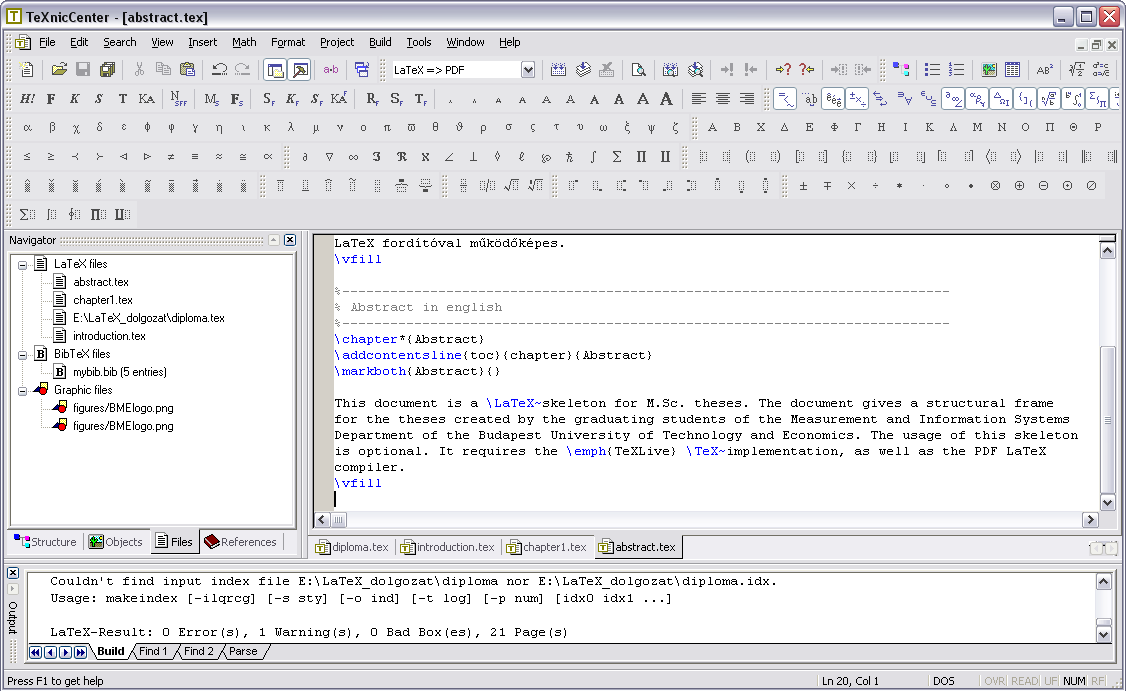
\includegraphics[width=150mm, keepaspectratio]{figures/TeXnicCenter.png}
\caption{A TeXnicCenter Windows alap� \LaTeX-szerkeszt�.} 
\label{fig:TexnicCenter}
\end{figure}

Egy m�sik haszn�lhat� Windows alap� szerkeszt�program a LEd (LaTeX Editor,\\\url{http://www.latexeditor.org/}), a TeXnicCenter azonban stabilabb, gyorsabb, �s jobban haszn�lhat�.

%----------------------------------------------------------------------------
\section{A dokumentum leford�t�sa Windows alatt}
%----------------------------------------------------------------------------
A TeXnicCenter �s a LEd kiz�r�lag szerkeszt�program (b�r az ut�bbiban DVI-n�zeget� is van), �gy a dokumentum ford�t�s�hoz sz�ks�ges eszk�z�ket nem tartalmazza. Windows alatt alapvet�en k�t lehet�s�g k�z�l �rdemes v�lasztani: MiKTeX (\url{http://miktex.org/}) �s TeXLive (\url{http://www.tug.org/texlive/}) programcsomag. Az ut�bbi m�k�dik Mac OS X, GNU/Linux alatt �s Unix-sz�rmaz�kokon is. A MiKTeX egy alapcsomag telep�t�se ut�n mindig let�lti a haszn�lt funkci�khoz sz�ks�ges, de lok�lisan hi�nyz� \TeX-csomagokat, m�g a TeXLive DVD ISO verz�ban f�rhet� hozz�. Ez a dokumentum TeXLive 2008 programcsomag seg�ts�g�vel fordult, amelynek DVD ISO verzi�ja a megadott oldalr�l let�lthet�. A sablon leford�t�s�hoz a disztrib�ci�ban szerepl� \verb+magyar.ldf+ f�jlt a \verb+http://www.math.bme.hu/latex/+ v�ltozatra kell cser�lni, vagy az ut�bbi v�ltozatot be kell m�solni a projekt-k�nyvt�rba (ahogy ezt meg is tett�k a sablonban) k�l�nben anom�li�k tapasztalhat�k a dokumentumban (pl. az �bra- �s t�bl�zat-al��r�sok form�tuma nem a be�ll�tott lesz, vagy bizonyos oldalakon megjelenik alap�telmez�sben egy fejl�c). A TeXLive 2008-at m�g nem kell k�l�n telep�teni a g�pre, elegend� DVD-r�l (vagy az ISO f�jlb�l k�zvetlen�l, pl. DaemonTools-szal) haszn�lni. 

A \TeX-eszk�z�ket tartalmaz� programcsomag bin�risainak el�r�si �tj�t minden esetben be kell �ll�tani a szerkeszt�programban, p�ld�ul TeXnicCenter eset�n legegyszer�bben a \verb+Build / Define output profiles...+ men�ponttal el�h�vott dial�gusablakban a \verb+Wizard...+ gombra kattintva tehetj�k ezt meg.

A PDF-\LaTeX~haszn�lata eset�n a gener�lt dokumentum k�zvetlen�l PDF-form�tumban �ll rendelkez�sre. Amennyiben a PDF-f�jl egy PDF-n�z�ben (pl. Adobe Acrobat Reader vagy Foxit PDF Reader) meg van nyitva, akkor a f�jlle�r�t a PDF-n�z� program tipikusan lefoglalja. Ilyen esetben a dokumentum �jraford�t�sa hiba�zenettel kil�p. Ha bez�rjuk �s �jra megnyitjuk a PDF dokumentumot, akkor pedig a PDF-n�z�k t�bbs�ge az els� oldalon nyitja meg a dokumentumot, nem a legut�bb olvasott oldalon. Ezzel szemben p�ld�ul az egyszer� �s ingyenes \textcolor{blue}{Sumatra PDF} nev� program k�pes arra, hogy a megnyitott dokumentum megv�ltoz�s�t detekt�lja, �s friss�tse a n�zetet az aktu�lis oldal megtart�s�val.

%----------------------------------------------------------------------------
\section{Eszk�z�k Linuxhoz}
%----------------------------------------------------------------------------
Linux oper�ci�s rendszer alatt is rengeteg szerkeszt�program van, pl. a KDE alap� Kile j�l haszn�lhat�. Ez ingyenesen let�lthet�, vagy �ppens�ggel az adott Linux-disztrib�ci� eleve tartalmazza, ahogyan a dokumentum ford�t�s�hoz sz�ks�ges csomagokat is. Az Ubuntu Linux disztrib�ci�k alatt p�ld�ul legt�bbsz�r a \verb+texlive-base+ csomag telep�t�s�vel haszn�lhat�k a \LaTeX-eszk�z�k.

%----------------------------------------------------------------------------
\chapter{A dolgozat formai kivitele}
%----------------------------------------------------------------------------
Az itt található információk egy része a BME VIK Hallgatói Képviselet által készített ,,Utolsó félév a villanykaron'' c. munkából lett kis változtatásokkal átemelve. Az eredeti dokumentum az alábbi linken érhető el: \url{http://vik-hk.bme.hu/diplomafelev-howto-2009}.

%----------------------------------------------------------------------------
\section{A dolgozat kimérete}
%----------------------------------------------------------------------------
A minimális 50, az optimális kiméret 60-70 oldal (függelékkel együtt). A bírálók és a záróvizsga bizottság sem szereti kifejezetten a túl hosszú dolgozatokat, így a bruttó 90 oldalt már nem érdemes túlszárnyalni. Egyébként függetlenül a dolgozat kiméretétől, ha a dolgozat nem érdekfeszítő, akkor az olvasó már az elején a végét fogja várni. Érdemes zárt, önmagában is érthető művet alkotni.

%----------------------------------------------------------------------------
\section{A dolgozat nyelve}
%----------------------------------------------------------------------------
Mivel Magyarországon a hivatalos nyelv a magyar, ezért alapértelmezésben magyarul kell megírni a dolgozatot. Aki külföldi posztgraduális képzésben akar részt venni, nemzetközi szintű tudományos kutatást szeretne végezni, vagy multinacionális cégnél akar elhelyezkedni, annak célszerű angolul megírnia diplomadolgozatát. Mielőtt a hallgató az angol nyelvű verzió mellett dönt, erősen ajánlott mérlegelni, hogy ez mennyi többletmunkát fog a hallgatónak jelenteni fogalmazás és nyelvhelyesség terén, valamint - nem utolsó sorban - hogy ez mennyi többletmunkát fog jelenteni a konzulens illetve bíráló számára. Egy nehezen olvasható, netalán érthetetlen szöveg teher minden játékos számára.

%----------------------------------------------------------------------------
\section{A dokumentum nyomdatechnikai kivitele}
%----------------------------------------------------------------------------
A dolgozatot A4-es fehér lapra nyomtatva, 2,5 centiméteres margóval (+1~cm kötésbeni), 11-12 pontos betűmérettel, talpas betűtípussal és másfeles sorközzel célszerű elkészíteni.



%----------------------------------------------------------------------------
\chapter{A \LaTeX-sablon használata}
%----------------------------------------------------------------------------
Ebben a fejezetben röviden, implicit módon bemutatjuk a sablon használatának módját, ami azt jelenti, hogy sablon használata ennek a dokumentumnak a forráskódját tanulmányozva válik teljesen világossá. Amennyiben a szoftver-keretrendszer telepítve van, a sablon alkalmazása és a dolgozat szerkesztése \LaTeX-ben a sablon segítségével tapasztalataink szerint jóval hatékonyabb, mint egy WYSWYG (\emph{What You See is What You Get}) típusú szövegszerkesztő esetén (pl. Microsoft Word, OpenOffice).

%----------------------------------------------------------------------------
\section{Címkék és hivatkozások}
%----------------------------------------------------------------------------
A \LaTeX~dokumentumban címkéket (\verb+\label+) rendelhetünk ábrákhoz, táblázatokhoz, fejezetekhez, listákhoz, képletekhez stb. Ezekre a dokumentum bármely részében hivatkozhatunk, a hivatkozások automatikusan feloldásra kerülnek.

A sablonban makrókat definiáltunk a hivatkozások megkönnyítéséhez. Ennek megfelelően minden ábra (\emph{figure}) címkéje \verb+fig:+ kulcsszóval kezdődik, míg minden táblázat (\emph{table}), képlet (\emph{equation}), fejezet (\emph{section}) és lista (\emph{listing}) rendre a \verb+tab:+, \verb+eq:+, \verb+sect:+ és \verb+listing:+ kulcsszóval kezdődik, és a kulcsszavak után tetszőlegesen választott címke használható. Ha ezt a konvenciót betartjuk, akkor az előbbi objektumok számára rendre a \verb+\figref+, \verb+\tabref+, \verb+\eqref+, \verb+\sectref+ és \verb+\listref+ makrókkal hivatkozhatunk. A makrók paramétere a címke, amelyre hivatkozunk (a kulcsszó nélkül). Az összes említett hivatkozástípus, beleértve az \verb+\url+ kulcsszóval bevezetett web-hivatkozásokat is a  \verb+hyperref+\footnote{Segítségével a dokumentumban megjelenő hivatkozások nem csak dinamikussá válnak, de színezhetők is, bővebbet erről a csomag dokumentációjában találunk. Ez egyúttal egy példa lábjegyzet írására.} csomagnak köszönhetően aktívak a legtöbb PDF-nézegetőben, rájuk kattintva a dokumentum megfelelő oldalára ugrik a PDF-néző vagy a megfelelő linket megnyitja az alapértelmezett böngészővel. A \verb+hyperref+ csomag a kimeneti PDF-dokumentumba könyvjelzőket is készít a tartalomjegyzékből. Ez egy szintén aktív tartalomjegyzék, amelynek elemeire kattintva a nézegető behozza a kiválasztott fejezetet.

%----------------------------------------------------------------------------
\section{Ábrák és táblázatok}
%----------------------------------------------------------------------------
A képeket PDFLaTeX esetén a veszteségmentes PNG, valamint a veszteséges JPEG formátumban érdemes elmenteni. Az EPS (PostScript) vektorgrafikus képformátum beillesztését a PDFLatex közvetlenül nem támogatja. Ehelyett egy lehetőség 200 dpi, vagy annál nagyobb felbontásban raszterizálni a képet, és PNG formátumban elmenteni. Az egyes képek mérete általában nem, de sok kép esetén a dokumentum összmérete így már szignifikáns is lehet. A dokumentumban felhasznált képfájlokat a dokumentum forrása mellett érdemes tartani, archiválni, mivel ezek hiányában a dokumentum nem fordul újra. Ha lehet, a vektorgrafikus képeket vektorgrafikus formátumban is érdemes elmenteni az újrafelhasználhatóság (az átszerkeszthetőség) érdekében.

Kapcsolási rajzok legtöbbször kimásolhatók egy vektorgrafikus programba (pl. CorelDraw) és onnan nagyobb felbontással raszterizálva kimenthatők PNG formátumban. Ugyanakkor kiváló ábrák készíthetők Microsoft Visio vagy hasonló program használatával is: Visio-ból az ábrák közvetlenül PNG-be is menthetők.

Lehetőségeink Matlab ábrák esetén:
\begin{itemize}
	\item Képernyőlopás (\emph{screenshot}) is elfogadható minőségű lehet a dokumentumban, de általában jobb felbontást is el lehet érni más módszerrel.
	\item A Matlab ábrát a \verb+File/Save As+ opcióval lementhetjük PNG formátumban (ugyanaz itt is érvényes, mint korábban, ezért nem javasoljuk).
	\item A Matlab ábrát az \verb+Edit/Copy figure+ opcióval kimásolhatjuk egy vektorgrafikus programba is és onnan nagyobb felbontással raszterizálva kimenthatjük PNG formátumban (nem javasolt).
	\item Javasolt megoldás: az ábrát a \verb+File/Save As+ opcióval EPS \emph{vektorgrafikus} formátumban elmentjük, PDF-be konvertálva beillesztjük a dolgozatba.
\end{itemize}
Az EPS kép az \verb+epstopdf+ programmal\footnote{a korábban említett \LaTeX-disztribúciókban megtalálható} konvertálható PDF formátumba. Célszerű egy batch-fájlt készíteni az összes EPS ábra lefordítására az alábbi módon (ez Windows alatt működik).
\begin{lstlisting}[frame=single,float=!ht]
@echo off
for %%j in (*.eps) do (
echo converting file "%%j"
epstopdf "%%j"
)
echo done .
\end{lstlisting}

Egy ilyen parancsfájlt (\verb+convert.cmd+) elhelyeztük a sablon \verb+figures\eps+ könyvtárába, így a felhasználónak csak annyi a dolga, hogy a \verb+figures\eps+ könyvtárba kimenti az EPS formátumú vektorgrafikus képet, majd lefuttatja a \verb+convert.cmd+ parancsfájlt, ami PDF-be konvertálja az EPS fájlt.

Ezek után a PDF-ábrát ugyanúgy lehet a dokumentumba beilleszteni, mint a PNG-t vagy a JPEG-et. A megoldás előnye, hogy a lefordított dokumentumban is vektorgrafikusan tárolódik az ábra, így a mérete jóval kisebb, mintha raszterizáltuk volna beillesztés előtt. Ez a módszer minden -- az EPS formátumot ismerő -- vektorgrafikus program (pl. CorelDraw) esetén is használható.

A képek beillesztésére az \sectref{LatexTools}. fejezetben mutattunk be példát (\figref{TexnicCenter}~ábra). Az előző mondatban egyúttal az automatikusan feloldódó ábrahivatkozásra is láthatunk példát. Több képfájlt is beilleszthetünk egyetlen ábrába. Az egyes képek közötti horizontális és vertikális margót metrikusan szabályozhatjuk (\figref{HVSpaces}~ábra). Az ábrák elhelyezését számtalan tipográfiai szabály egyidejű teljesítésével a fordító maga végzi, a dokumentum írója csak preferenciáit jelezheti a fordító felé (olykor ez bosszúságot is okozhat, ilyenkor pl. a kép méretével lehet játszani).

\begin{figure}[!ht]
\centering
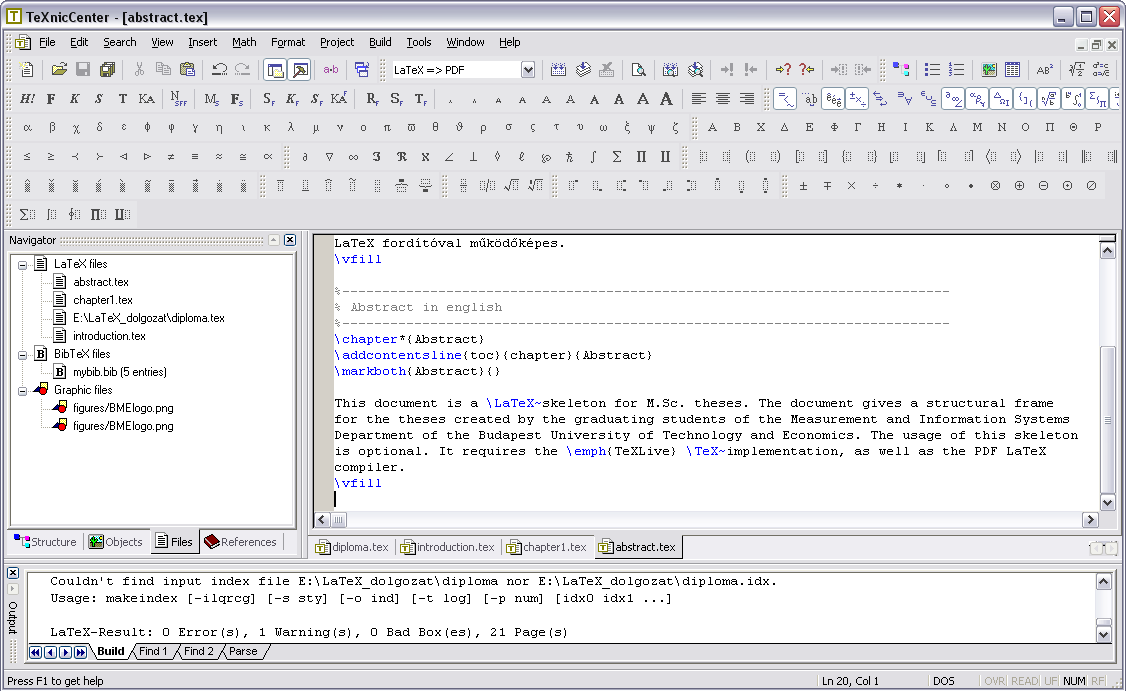
\includegraphics[width=67mm, keepaspectratio]{figures/TeXnicCenter.png}\hspace{1cm}
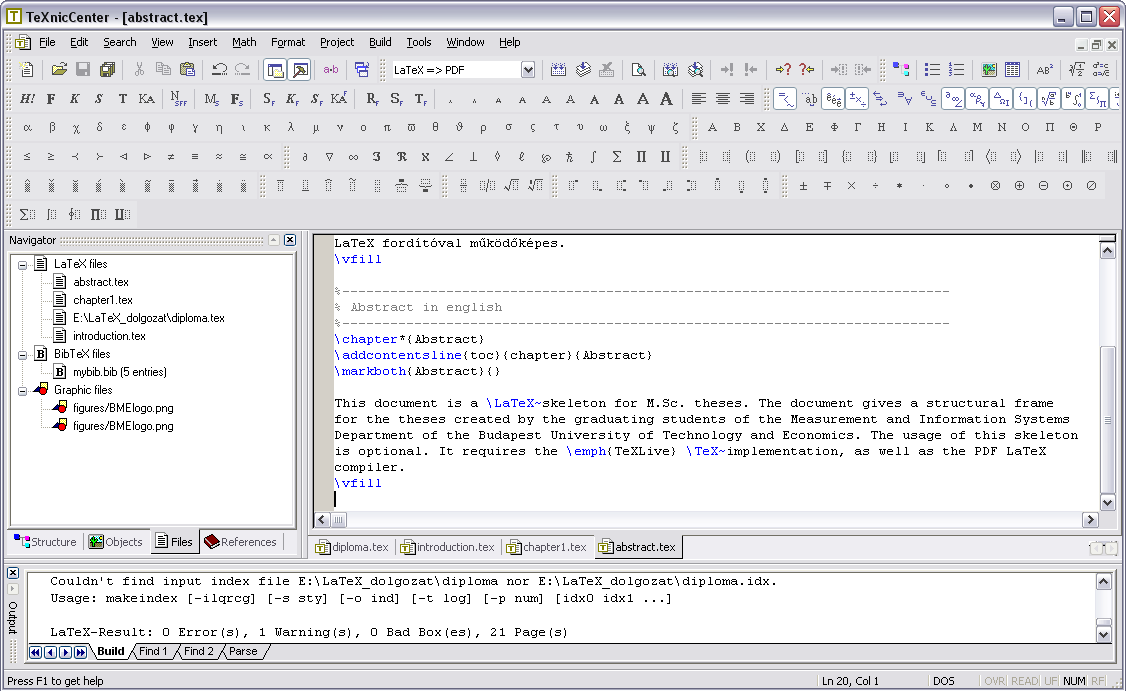
\includegraphics[width=67mm, keepaspectratio]{figures/TeXnicCenter.png}\\\vspace{5mm}
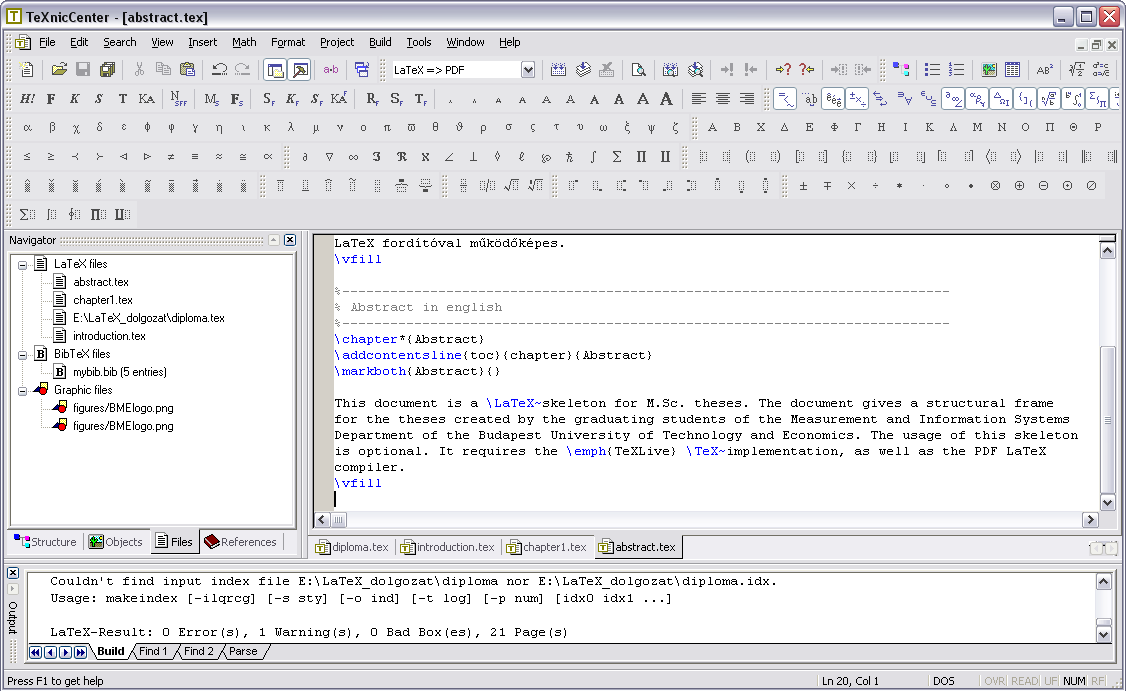
\includegraphics[width=67mm, keepaspectratio]{figures/TeXnicCenter.png}\hspace{1cm}
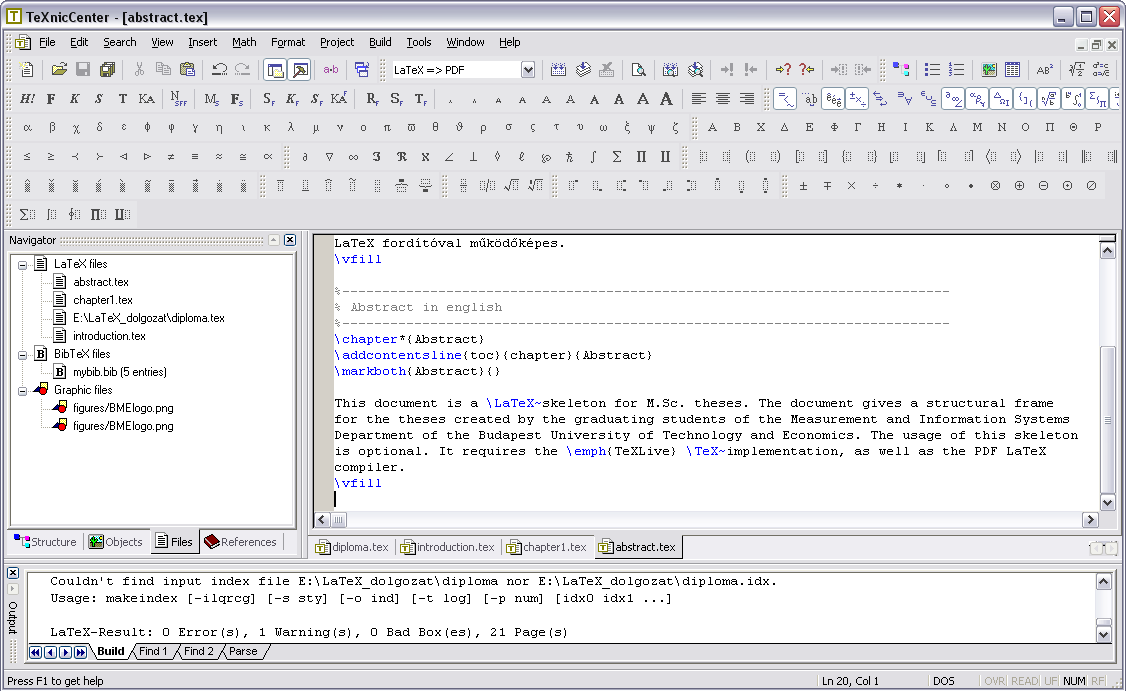
\includegraphics[width=67mm, keepaspectratio]{figures/TeXnicCenter.png}
\caption{Több képfájl beillesztése esetén térközöket is érdemes használni.} 
\label{fig:HVSpaces}
\end{figure}

A táblázatok használatára a \tabref{TabularExample}~táblázat mutat példát.
A táblázat címkéje nem véletlenül került a táblázat fölé, ez a szokványos.
\begin{table}[ht]
	\footnotesize
	\centering
	\caption{Az órajel-generátor chip órajel-kimenetei.} \label{tab:SysClocks}
	\begin{tabular}{ | l | c | c |}
	\hline
	Órajel & Frekvencia & Cél pin \\ \hline
	CLKA & 100 MHz & FPGA CLK0\\
	CLKB & 48 MHz  & FPGA CLK1\\
	CLKC & 20 MHz  & Processzor\\
	CLKD & 25 MHz  & Ethernet chip \\
	CLKE & 72 MHz  & FPGA CLK2\\
	XBUF & 20 MHz  & FPGA CLK3\\
	\hline
	\end{tabular}
	\label{tab:TabularExample}
\end{table}


%----------------------------------------------------------------------------
\section{Felsorolások és listák}
%----------------------------------------------------------------------------
Számozatlan felsorolásra mutat példát a jelenlegi bekezdés:
\begin{itemize}
	\item \emph{első bajusz:} ide lehetne írni az első elem kifejését,
	\item \emph{második bajusz:} ide lehetne írni a második elem kifejését,
	\item \emph{ez meg egy szakáll:} ide lehetne írni a harmadik elem kifejését.
\end{itemize}

Számozott felsorolást is készíthetünk az alábbi módon:
\begin{enumerate}
	\item \emph{első bajusz:} ide lehetne írni az első elem kifejését, és ez a kifejtés így néz ki, ha több sorosra sikeredik,
	\item \emph{második bajusz:} ide lehetne írni a második elem kifejését,
	\item \emph{ez meg egy szakáll:} ide lehetne írni a harmadik elem kifejését.
\end{enumerate}
A felsorolásokban sorok végén vessző, az utolsó sor végén pedig pont a szokásos írásjel. Ez alól kivételt képezhet, ha az egyes elemek több teljes mondatot tartalmaznak.

Listákban a dolgozat szövegétől elkülönítendő kódrészleteket, programsorokat, pszeudo-kódokat jeleníthetünk meg (\listref{Example}~lista). 
\begin{lstlisting}[frame=single,float=!ht,caption=A fenti számozott felsorolás \LaTeX- forráskódja, label=listing:Example]
\begin{enumerate}
	\item \emph{első bajusz:} ide lehetne írni az első elem kifejését, 
	és ez a kifejtés így néz ki, ha több sorosra sikeredik,
	\item \emph{második bajusz:} ide lehetne írni a második elem kifejését,
	\item \emph{ez meg egy szakáll:} ide lehetne írni a harmadik elem kifejését.
\end{enumerate}
\end{lstlisting}
A lista keretét, háttérszínét, egész stílusát megválaszthatjuk. Ráadásul különféle programnyelveket és a nyelveken belül kulcsszavakat is definiálhatunk, ha szükséges. Erről bővebbet a \verb+listings+ csomag hivatalos leírásában találhatunk.

%----------------------------------------------------------------------------
\section{Képletek}
%----------------------------------------------------------------------------
Ha egy formula nem túlságosan hosszú, és nem akarjuk hivatkozni a szövegből, mint például a $e^{i\pi}+1=0$ képlet, \emph{szövegközi képletként} szokás leírni. Csak, hogy másik példát is lássunk, az $U_i=-d\Phi/dt$ Faraday-törvény a $\rot E=-\frac{dB}{dt}$ differenciális alakban adott Maxwell-egyenlet felületre vett integráljából vezethető le. Látható, hogy a \LaTeX-fordító a sorközöket betartja, így a szöveg szedése esztétikus marad szövegközi képletek használata esetén is.

Képletek esetén az általános konvenció, hogy a kisbetűk skalárt, a kis félkövér betűk ($\mathbf{v}$) oszlopvektort -- és ennek megfelelően $\mathbf{v}^T$ sorvektort -- a kapitális félkövér betűk ($\mathbf{V}$) mátrixot jelölnek. Ha ettől el szeretnénk térni, akkor az alkalmazni kívánt jelölésmódot célszerű külön alfejezetben definiálni. Ennek megfelelően, amennyiben $\mathbf{y}$ jelöli a mérések vektorát, $\mathbf{\vartheta}$ a paraméterek vektorát és $\hat{\mathbf{y}}=\mathbf{X}\vartheta$ a paraméterekben lineáris modellt, akkor a \emph{Least-Squares} értelemben optimális paraméterbecslő $\hat{\mathbf{\vartheta}}_{LS}=(\mathbf{X}^T\mathbf{X})^{-1}\mathbf{X}^T\mathbf{y}$ lesz.

Emellett kiemelt, sorszámozott képleteket is megadhatunk, ennél az \verb+equation+ és a \verb+eqnarray+ környezetek helyett a korszerűbb \verb+align+ környezet alkalmazását javasoljuk (több okból, különféle problémák elkerülése végett, amelyekre most nem térünk ki). Tehát
\begin{align}
\dot{\mathbf{x}}&=\mathbf{A}\mathbf{x}+\mathbf{B}\mathbf{u},\\
\mathbf{y}&=\mathbf{C}\mathbf{x},
\end{align}
ahol $\mathbf{x}$ az állapotvektor, $\mathbf{y}$ a mérések vektora és $\mathbf{A}$, $\mathbf{B}$ és $\mathbf{C}$ a rendszert leíró paramétermátrixok. Figyeljük meg, hogy a két egyenletben az egyenlőségjelek egymáshoz igazítva jelennek meg, mivel a mindkettőt az \& karakter előzi meg a kódban. Lehetőség van számozatlan kiemelt képlet használatára is, például
\begin{align}
\dot{\mathbf{x}}&=\mathbf{A}\mathbf{x}+\mathbf{B}\mathbf{u},\nonumber\\
\mathbf{y}&=\mathbf{C}\mathbf{x}\nonumber.
\end{align}
Mátrixok felírására az $\mathbf{A}\mathbf{x}=\mathbf{b}$ inhomogén lineáris egyenlet részletes kifejtésével mutatunk példát:
\begin{align}
\begin{bmatrix}
a_{11} & a_{12} & \dots & a_{1n}\\
a_{21} & a_{22} & \dots & a_{2n}\\
\vdots & \vdots & \ddots & \vdots\\
a_{m1} & a_{m2} & \dots & a_{mn}
\end{bmatrix}
\begin{pmatrix}x_1\\x_2\\\vdots\\x_n\end{pmatrix}=
\begin{pmatrix}b_1\\b_2\\\vdots\\b_m\end{pmatrix}.
\end{align}
A \verb+\frac+ utasítás hatékonyságát egy általános másodfokú tag átviteli függvényén keresztül mutatjuk be, azaz
\begin{align}
W(s)=\frac{A}{1+2T\xi s+s^2T^2}.
\end{align}
A matematikai mód minden szimbólumának és képességének a bemutatására természetesen itt nincs lehetőség, de gyors referenciaként hatékonyan használhatók a következő linkek:\\
\indent\url{http://www.artofproblemsolving.com/LaTeX/AoPS_L_GuideSym.php},\\
\indent\url{http://www.ctan.org/tex-archive/info/symbols/comprehensive/symbols-a4.pdf},\\
\indent\url{ftp://ftp.ams.org/pub/tex/doc/amsmath/short-math-guide.pdf}.\\
Ez pedig itt egy magyarázat, hogy miért érdemes \verb+align+ környezetet használni:\\
\indent\url{http://texblog.net/latex-archive/maths/eqnarray-align-environment/}.

%----------------------------------------------------------------------------
\section{Irodalmi hivatkozások}\label{sect:HowtoReference}
%----------------------------------------------------------------------------
Egy \LaTeX dokumentumban az irodalmi hivatkozások definíciójának két módja van. Az egyik a \verb+\thebibliograhy+ környezet használata a dokumentum végén, az \verb+\end{document}+ lezárás előtt.
\begin{lstlisting}[frame=single,float=!ht]
\begin{thebibliography}{9}

\bibitem{Lamport94} Leslie Lamport, \emph{\LaTeX: A Document Preparation System}. 
Addison Wesley, Massachusetts, 2nd Edition, 1994.

\end{thebibliography}
\end{lstlisting}

Ezek után a dokumentumban a \verb+\cite{Lamport94}+ utasítással hivatkozhatunk a forrásra. A fenti megadás viszonylag kötetlen, a szerző maga formázza az irodalomjegyzéket. 

Egy sokkal professzionálisabb módszer a BiB\TeX~használata, ezért ez a sablon is ezt támogatja. Ebben az esetben egy külön szöveges adatbázisban definiáljuk a forrásmunkákat, és egy külön stílusfájl határozza meg az irodalomjegyzék kinézetét. Ez, összhangban azzal, hogy külön formátumkonvenció határozza meg a folyóirat-, a könyv-, a konferenciacikk- stb. hivatkozások kinézetét az irodalomjegyzékben (a sablon használata esetén ezzel nem is kell foglalkoznia a hallgatónak, de az eredményt célszerű ellenőrizni). A felhasznált hivatkozások adatbázisa egy \verb+.bib+ kiterjesztésű szöveges fájl, amelynek szerkezetét a \listref{Bibtex} kódrészlet demonstrálja. A forrásmunkák bevitelekor a sor végi vesszők külön figyelmet igényelnek, mert hiányuk a BiB\TeX-fordító hibaüzenetét eredményezi. A forrásmunkákat típus szerinti kulcsszó vezeti be (\verb+@book+ könyv, \verb+@inproceedings+ konferenciakiadványban megjelent cikk, \verb+@article+ folyóiratban megjelent cikk, \verb+@techreport+ valamelyik egyetem gondozásában megjelent műszaki tanulmány, \verb+@manual+ műszaki dokumentáció esetén stb.). Nemcsak a megjelenés stílusa, de a kötelezően megadandó mezők is típusról-típusra változnak. Egy jól használható referencia a \url{http://en.wikipedia.org/wiki/BibTeX} oldalon található.
\begin{lstlisting}[frame=single,float=!ht,caption=Példa szöveges irodalomjegyzék-adatbázisra BiBTeX használata esetén., label=listing:Bibtex]
@BOOK{Wettl04,
  author="Ferenc Wettl and Gyula Mayer and Péter Szabó",
  title="\LaTeX~kézikönyv",
  publisher="Panem Könyvkiadó",
  year=2004
}
@ARTICLE{Candy86,
  author ="James C. Candy",
  title  ="Decimation for Sigma Delta Modulation",
  journal="{IEEE} Trans.\ on Communications",
  volume =34,
  number =1,
  pages  ="72--76",
  month  =jan,
  year   =1986,
}
@INPROCEEDINGS{Lee87,
  author =       "Wai L. Lee and Charles G. Sodini",
  title =        "A Topology for Higher Order Interpolative Coders",
  booktitle =    "Proc.\ of the IEEE International Symposium on 
  Circuits and Systems",
  year =         1987,
  vol =          2,
  month =        may # "~4--7",
  address =      "Philadelphia, PA, USA",
  pages =        "459--462"
}
@PHDTHESIS{KissPhD,
  author =   "Peter Kiss",
  title =    "Adaptive Digital Compensation of Analog Circuit Imperfections 
  for Cascaded Delta-Sigma Analog-to-Digital Converters",
  school =   "Technical University of Timi\c{s}oara, Romania",
  month =    apr,
  year =     2000
}
@MANUAL{Schreier00,
  author = "Richard Schreier",
  title  = "The Delta-Sigma Toolbox v5.2",
  organization = "Oregon State University",
  year   = 2000,
  month  = jan,
  note   ="\newline URL: http://www.mathworks.com/matlabcentral/fileexchange/"
}
@MISC{DipPortal,
	author="Budapesti {M}űszaki és {G}azdaságtudományi {E}gyetem 
	{V}illamosmérnöki és {I}nformatikai {K}ar",
  title="{D}iplomaterv portál (2011 február 26.)",
  howpublished="\url{http://diplomaterv.vik.bme.hu/}",
}}
\end{lstlisting}

A stílusfájl egy \verb+.sty+ kiterjesztésű fájl, de ezzel lényegében nem kell foglalkozni, mert vannak beépített stílusok, amelyek jól használhatók. Ez a sablon a BiB\TeX-et használja, a hozzá tartozó adatbázisfájl a \verb+mybib.bib+ fájl. Megfigyelhető, hogy az irodalomjegyzéket a dokumentum végére (a \verb+\end{document}+ utasítás elé) beillesztett \verb+\bibliography{mybib}+ utasítással hozhatjuk létre, a stílusát pedig ugyanitt a  \verb+\bibliographystyle{plain}+ utasítással adhatjuk meg. Ebben az esetben a \verb+plain+ előre definiált stílust használjuk (a sablonban is ezt állítottuk be). A \verb+plain+ stíluson kívül természetesen számtalan más előre definiált stílus is létezik. Mivel a \verb+.bib+ adatbázisban ezeket megadtuk, a BiB\TeX-fordító is meg tudja különböztetni a szerzőt a címtől és a kiadótól, és ez alapján automatikusan generálódik az irodalomjegyzék a stílusfájl által meghatározott stílusban.

Az egyes forrásmunkákra a szövegből továbbra is a \verb+\cite+ paranccsal tudunk hivatkozni, így a \listref{Bibtex} kódrészlet esetén a hivatkozások rendre \verb+\cite{Wettl04}+, \verb+\cite{Candy86}+, \verb+\cite{Lee87}+, \verb+\cite{KissPhD}+, \verb+\cite{Schreirer00}+ és \verb+\cite{DipPortal}+. Az irodalomjegyzékben alapértelmezésben csak azok a forrásmunkák jelennek meg, amelyekre található hivatkozás a szövegben, és ez így alapvetően helyes is, hiszen olyan forrásmunkákat nem illik az irodalomjegyzékbe írni, amelyekre nincs hivatkozás.

Mivel a fordítási folyamat során több lépésben oldódnak fel a szimbólumok, ezért gyakran többször (TeXLive és TeXnicCenter esetén 2-3-szor) is le kell fordítani a dokumentumot. Ilyenkor ez első 1-2 fordítás esetleg szimbólum-feloldásra vonatkozó figyelmeztető üzenettel zárul. Ha hibaüzenettel zárul bármelyik fordítás, akkor nincs értelme megismételni, hanem a hibát kell megkeresni. A \verb+.bib+ fájl megváltoztatáskor sokszor nincs hatása a változtatásnak azonnal, mivel nem mindig fut újra a BibTeX fordító. Ezért célszerű a változtatás után azt manuálisan is lefuttatni (TeXnicCenter esetén \verb+Build/BibTeX+).

Hogy a szövegbe ágyazott hivatkozások kinézetét demonstráljuk, itt most sorban meghivatkozzuk a \cite{Wettl04}, \cite{Candy86}, \cite{Lee87}, \cite{KissPhD} és az \cite{Schreier00} forrásmunkát, valamint az \cite{DipPortal} weboldalt.

Megjegyzendő, hogy az ékezetes magyar betűket is tartalmazó \verb+.bib+ fájl az \verb+inputenc+ csomaggal betöltött \verb+latin2+ betűkészlet miatt fordítható. Ugyanez a \verb+.bib+ fájl hibaüzenettel fordul egy olyan dokumentumban, ami nem tartalmazza a \verb+\usepackage[latin2]{inputenc}+ sort. Speciális igény esetén az irodalmi adatbázis általánosabb érvényűvé tehető, ha az ékezetes betűket speciális latex karakterekkel helyettesítjük a \verb+.bib+ fájlban, pl. á helyett \verb+\'{a}+-t vagy ő helyett \verb+\H{o}+-t írunk. 

Oldaltörés következik (ld. forrás).
\newpage

%----------------------------------------------------------------------------
\section{A dolgozat szerkezete és a forrásfájlok}
%----------------------------------------------------------------------------
A diplomatervsablon (a kari irányelvek szerint) az alábbi fő fejezetekből áll:
\begin{enumerate}
	\item 1 oldalas \emph{tájékoztató} a szakdolgozat/diplomaterv szerkezetéről (\verb+guideline.tex+), ami a végső dolgozatból törlendő,
	\item \emph{feladatkiírás} (\verb+project.tex+), a dolgozat nyomtatott verzójában ennek a helyére kerül a tanszék által kiadott, a tanszékvezető által aláírt feladatkiírás, a dolgozat elektronikus verziójába pedig a feladatkiírás egyáltalán ne kerüljön bele, azt külön tölti fel a tanszék a diplomaterv-honlapra,
	\item \emph{címoldal} (\verb+titlepage.tex+),
	\item \emph{tartalomjegyzék} (\verb+diploma.tex+),
	\item a diplomatervező \emph{nyilatkozat}a az önálló munkáról (\verb+declaration.tex+),
	\item 1-2 oldalas tartalmi \emph{összefoglaló} magyarul és angolul, illetve elkészíthető még további nyelveken is (\verb+abstract.tex+),
	\item \emph{bevezetés}: a feladat értelmezése, a tervezés célja, a feladat indokoltsága, a diplomaterv felépítésének rövid összefoglalása (\verb+introduction.tex+),
	\item sorszámmal ellátott \emph{fejezetek}: a feladatkiírás pontosítása és részletes elemzése, előzmények (irodalomkutatás, hasonló alkotások), az ezekből levonható következtetések, a tervezés részletes leírása, a döntési lehetőségek értékelése és a választott megoldások indoklása, a megtervezett műszaki alkotás értékelése, kritikai elemzése, továbbfejlesztési lehetőségek (\verb+chapter{1,2..n}.tex+),
	\item esetleges \emph{köszönetnyilvánítás}ok (\verb+acknowledgement.tex+),
	\item részletes és pontos \emph{irodalomjegyzék} (ez a sablon esetében automatikusan generálódik a \verb+diploma.tex+ fájlban elhelyezett \verb+\bibliography+ utasítás hatására, a \sectref{HowtoReference}. fejezetben leírtak szerint),
	\item \emph{függelékek} (\verb+appendices.tex+).
\end{enumerate}

A sablonban a fejezetek a \verb+diploma.tex+ fájlba vannak beillesztve \verb+\include+ utasítások segítségével. Lehetőség van arra, hogy csak az éppen szerkesztés alatt álló \verb+.tex+ fájlt fordítsuk le, ezzel lerövidítve a fordítási folyamatot. Ezt a lehetőséget az alábbi kódrészlet biztosítja a \verb+diploma.tex+ fájlban.
\begin{lstlisting}[frame=single,float=!ht]
\includeonly{
	guideline,%
	project,%
	titlepage,%
	declaration,%
	abstract,%
	introduction,%
	chapter1,%
	chapter2,%
	chapter3,%
	acknowledgement,%
	appendices,%
}
\end{lstlisting}

Ha az alábbi kódrészletben az egyes sorokat a \verb+%+ szimbólummal kikommentezzük, akkor a megfelelő \verb+.tex+ fájl nem fordul le. Az oldalszámok és a tartalomjegyék természetesen csak akkor billennek helyre, ha a teljes dokumentumot lefordítjuk.

%----------------------------------------------------------------------------
\newpage
\section{Alapadatok megadása}
%----------------------------------------------------------------------------
A diplomaterv alapadatait (cím, szerző, konzulens, konzulens titulusa) a \verb+diploma.tex+ fájlban lehet megadni az alábbi kódrészlet módosításával.
\begin{lstlisting}[frame=single,float=!ht]
\newcommand{\vikszerzo}{Bódis-Szomorú András}
\newcommand{\vikkonzulens}{dr.~Konzulens Elemér}
\newcommand{\vikcim}{Elektronikus terelők}
\newcommand{\viktanszek}{Méréstechnika és Információs Rendszerek Tanszék}
\newcommand{\vikdoktipus}{Diplomaterv}
\end{lstlisting}

%----------------------------------------------------------------------------
\section{Új fejezet írása}
%----------------------------------------------------------------------------
A főfejezetek külön \verb+chapter{1..n}.tex+ fájlban foglalnak helyet. A sablonhoz 3 fejezet készült. További főfejezeteket úgy hozhatunk létre, ha új \verb+chapter{i}.tex+ fájlt készítünk a fejezet számára, és a \verb+diploma.tex+ fájlban, a \verb+\include+ és \verb+\includeonly+ utasítások argumentumába felvesszük az új \verb+.tex+ fájl nevét.






%----------------------------------------------------------------------------
\chapter*{\koszonetnyilvanitas}\addcontentsline{toc}{chapter}{\koszonetnyilvanitas}
%----------------------------------------------------------------------------

Ez nem kötelező, akár törölhető is. Ha a szerző szükségét érzi, itt lehet köszönetet nyilvánítani azoknak, akik hozzájárultak munkájukkal ahhoz, hogy a hallgató a szakdolgozatban vagy diplomamunkában leírt feladatokat sikeresen elvégezze. A konzulensnek való köszönetnyilvánítás sem kötelező, a konzulensnek hivatalosan is dolga, hogy a hallgatót konzultálja.

%\listoffigures\addcontentsline{toc}{chapter}{Ábrák jegyzéke}
%\listoftables\addcontentsline{toc}{chapter}{Táblázatok jegyzéke}

\bibliography{bib/mybib}
\addcontentsline{toc}{chapter}{Irodalomjegyzék}
\bibliographystyle{plain}

%----------------------------------------------------------------------------
\appendix
%----------------------------------------------------------------------------
\chapter*{F�ggel�k}\addcontentsline{toc}{chapter}{F�ggel�k}
\setcounter{chapter}{6}  % a fofejezet-szamlalo az angol ABC 6. betuje (F) lesz
\setcounter{equation}{0} % a fofejezet-szamlalo az angol ABC 6. betuje (F) lesz
\numberwithin{equation}{section}
\numberwithin{figure}{section}
\numberwithin{lstlisting}{section}
%\numberwithin{tabular}{section}

%----------------------------------------------------------------------------
\section{A TeXnicCenter fel�lete}
%----------------------------------------------------------------------------
\begin{figure}[!ht]
\centering
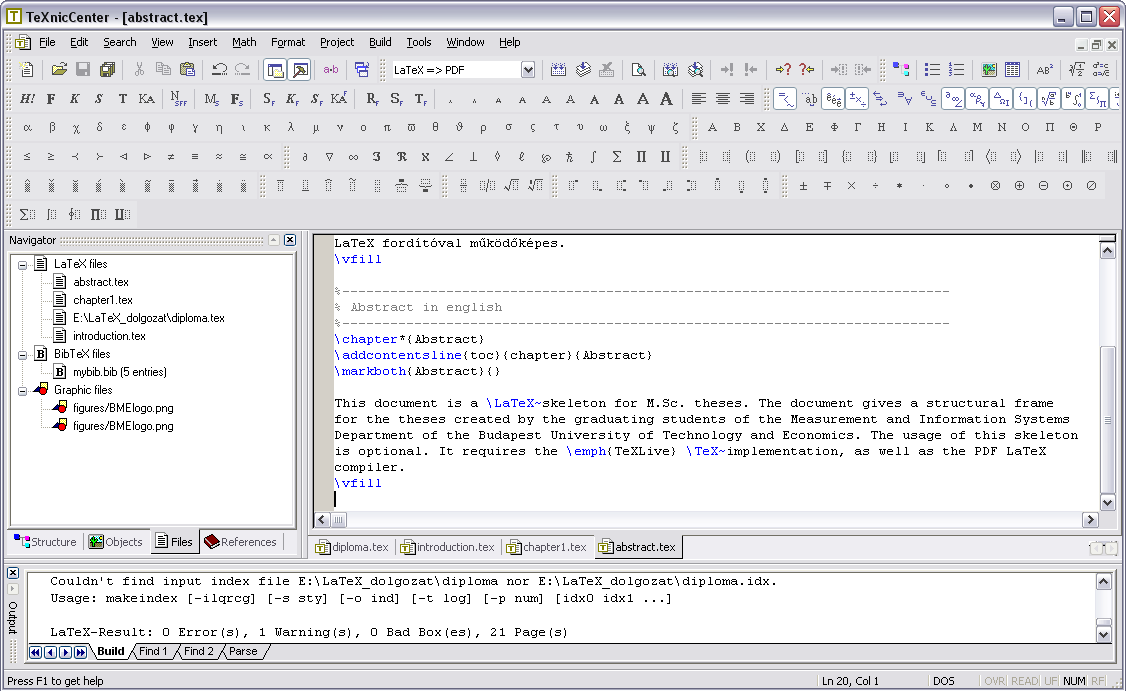
\includegraphics[width=150mm, keepaspectratio]{figures/TeXnicCenter.png}
\caption{A TeXnicCenter Windows alap� \LaTeX-szerkeszt�.} 
\end{figure}

%----------------------------------------------------------------------------
\clearpage\section{V�lasz az ,,�let, a vil�gmindens�g, meg minden'' k�rd�s�re}
%----------------------------------------------------------------------------
A Pitagorasz-t�telb�l levezetve
\begin{align}
c^2=a^2+b^2=42.
\end{align}
A Faraday-indukci�s t�rv�nyb�l levezetve
\begin{align}
\rot E=-\frac{dB}{dt}\hspace{1cm}\longrightarrow \hspace{1cm}
U_i=\oint\limits_\mathbf{L}{\mathbf{E}\mathbf{dl}}=-\frac{d}{dt}\int\limits_A{\mathbf{B}\mathbf{da}}=42.
\end{align}







\label{page:last}
\end{document}
